
%(BEGIN_QUESTION)
% Copyright 2010, Tony R. Kuphaldt, released under the Creative Commons Attribution License (v 1.0)
% This means you may do almost anything with this work of mine, so long as you give me proper credit

A motor controlled by a PLC refuses to start when the ``Start'' pushbutton switch is pressed.  A fellow instrument technician reports seeing the LED indicator for channel Y1 on the output card illuminated, but does not report on the illumination status of any other LEDs on the PLC.  Shown here is a partial wiring diagram and offline PLC program display for the system:

$$\includegraphics[width=15.5cm]{i02251x01.eps}$$

\vskip 10pt

Identify the likelihood of each specified fault in this system.  Consider each fault one at a time (i.e. no coincidental faults), determining whether or not each fault could independently account for {\it all} observations and symptoms in this circuit.

% No blank lines allowed between lines of an \halign structure!
% I use comments (%) instead, so that TeX doesn't choke.

$$\vbox{\offinterlineskip
\halign{\strut
\vrule \quad\hfil # \ \hfil & 
\vrule \quad\hfil # \ \hfil & 
\vrule \quad\hfil # \ \hfil \vrule \cr
\noalign{\hrule}
%
% First row
{\bf Fault} & {\bf Possible} & {\bf Impossible} \cr
%
\noalign{\hrule}
%
% Another row
Start pushbutton switch failed open &  &  \cr
%
\noalign{\hrule}
%
% Another row
Stop pushbutton switch failed open &  &  \cr
%
\noalign{\hrule}
%
% Another row
Start pushbutton switch failed shorted &  &  \cr
%
\noalign{\hrule}
%
% Another row
Stop pushbutton switch failed shorted &  &  \cr
%
\noalign{\hrule}
%
% Another row
Contactor coil failed open &  &  \cr
%
\noalign{\hrule}
%
% Another row
Bit {\tt X2} forced to a ``0'' state in the PLC &  &  \cr
%
\noalign{\hrule}
%
% Another row
Bit {\tt Y1} forced to a ``1'' state in the PLC &  &  \cr
%
\noalign{\hrule}
} % End of \halign 
}$$ % End of \vbox

\underbar{file i02251}
%(END_QUESTION)





%(BEGIN_ANSWER)

% No blank lines allowed between lines of an \halign structure!
% I use comments (%) instead, so that TeX doesn't choke.

$$\vbox{\offinterlineskip
\halign{\strut
\vrule \quad\hfil # \ \hfil & 
\vrule \quad\hfil # \ \hfil & 
\vrule \quad\hfil # \ \hfil \vrule \cr
\noalign{\hrule}
%
% First row
{\bf Fault} & {\bf Possible} & {\bf Impossible} \cr
%
\noalign{\hrule}
%
% Another row
Start pushbutton switch failed open &  & $\surd$ \cr
%
\noalign{\hrule}
%
% Another row
Stop pushbutton switch failed open &  & $\surd$ \cr
%
\noalign{\hrule}
%
% Another row
Start pushbutton switch failed shorted &  & $\surd$ \cr
%
\noalign{\hrule}
%
% Another row
Stop pushbutton switch failed shorted &  & $\surd$ \cr
%
\noalign{\hrule}
%
% Another row
Contactor coil failed open & $\surd$ &  \cr
%
\noalign{\hrule}
%
% Another row
Bit {\tt X2} forced to a ``0'' state in the PLC &  & $\surd$ \cr
%
\noalign{\hrule}
%
% Another row
Bit {\tt Y1} forced to a ``1'' state in the PLC &  & $\surd$ \cr
%
\noalign{\hrule}
} % End of \halign 
}$$ % End of \vbox


%(END_ANSWER)





%(BEGIN_NOTES)

{\bf This question is intended for exams only and not worksheets!}.

%(END_NOTES)

